Die Abbildungen \ref{fig:Grafana_Gain0}-\ref{fig:Grafana_Gain3} zeigen die gleiche Messung eines wolkenfreien Dezembertages am 12.12.2020 in Berlin mit unterschiedlichen Verstärkungsfaktoren. Der Integrationswert ist auf 255 gesetzt.\\
Es ist zu erkennen, dass die Auflösung der Y-Achse mit zunehmender Verstärkung (Gain) steigt. Aus Abbildung \ref{fig:Grafana_Gain3} ist jedoch ersichtlich, dass der maximale Messwert von 65.000 mit einem hohen Verstärkungsfaktor erreicht werden kann und die Daten so ihre Aussagekraft verlieren (clipping).
Abbildung \ref{fig:Grafana_AutoGain} zeigt die gleiche Messung im AutoGain-Modus. 
In diesem Plot werden immer die Messwerte mit dem größtmöglichen Verstärkungsfaktor zusammengefasst, bei dem es nicht zu clipping kommt.
Die Ausgabedaten der Messung sind nicht kalibriert und haben keine Einheit. Bei festem Gain liegen sie zwischen 0 und 65000.
Im AutoGain-Modus liegen sie zwischen 0 und 4160000.
Um die Daten nutzbar zu machen, müssen sie mithilfe eines anderen Messgerätes auf allgemein verständliche Werte kalibriert werden.

\begin{figure}[H]
  \begin{subfigure}[b]{0.5\textwidth}
    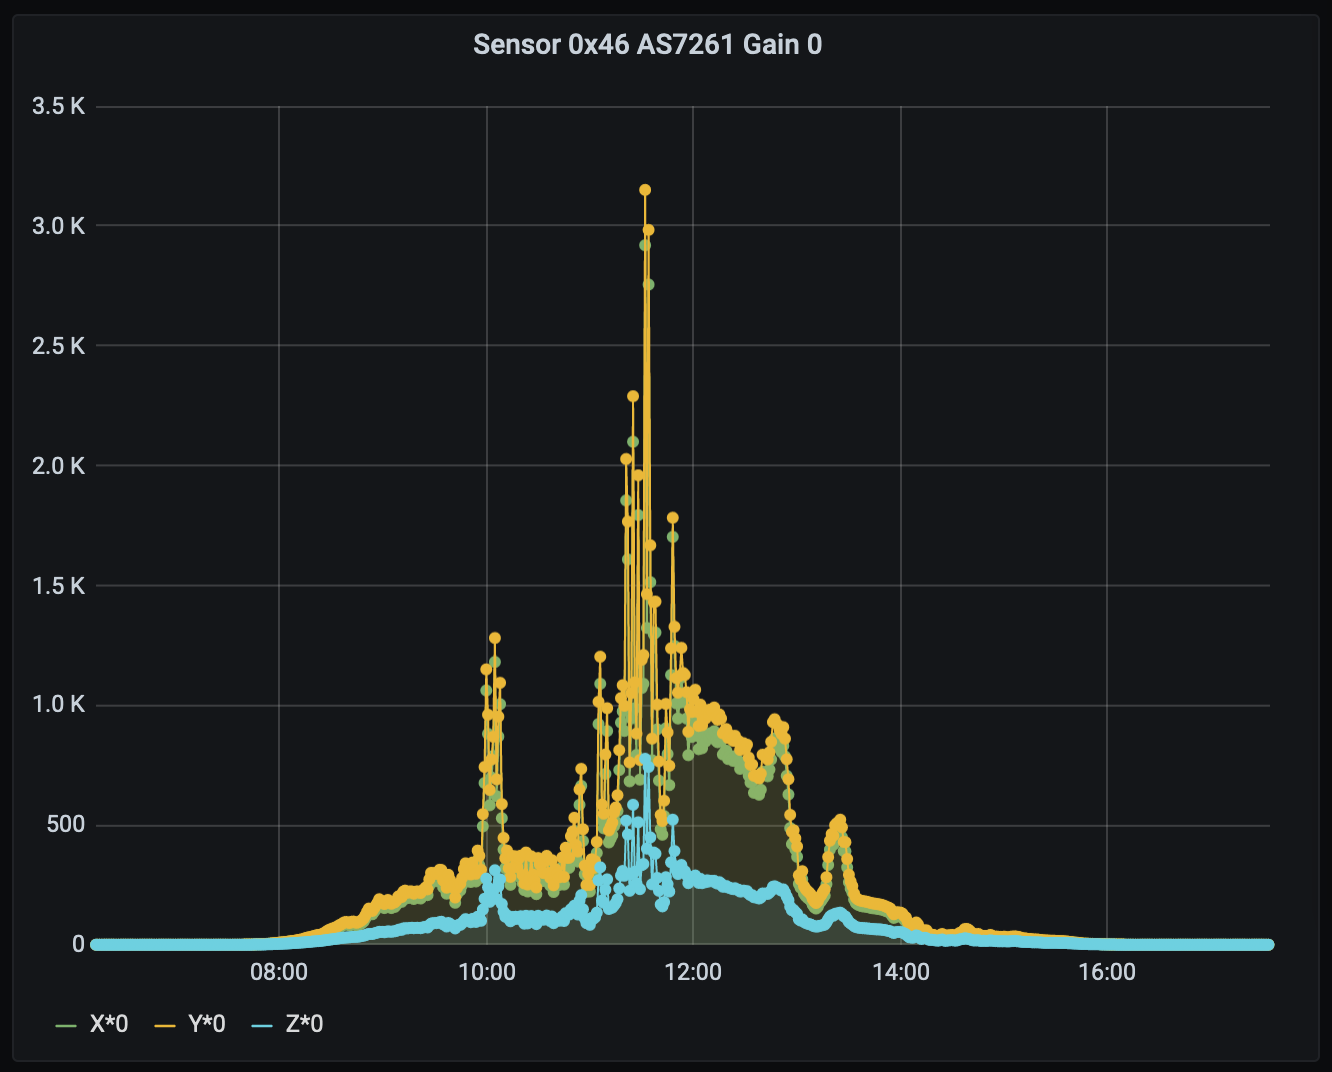
\includegraphics[width=\textwidth]{img/Grafana-Gain0}
    \caption{Gain 0 (1x)}
	\label{fig:Grafana_Gain0}
  \end{subfigure}
  %
  \begin{subfigure}[b]{0.5\textwidth}
    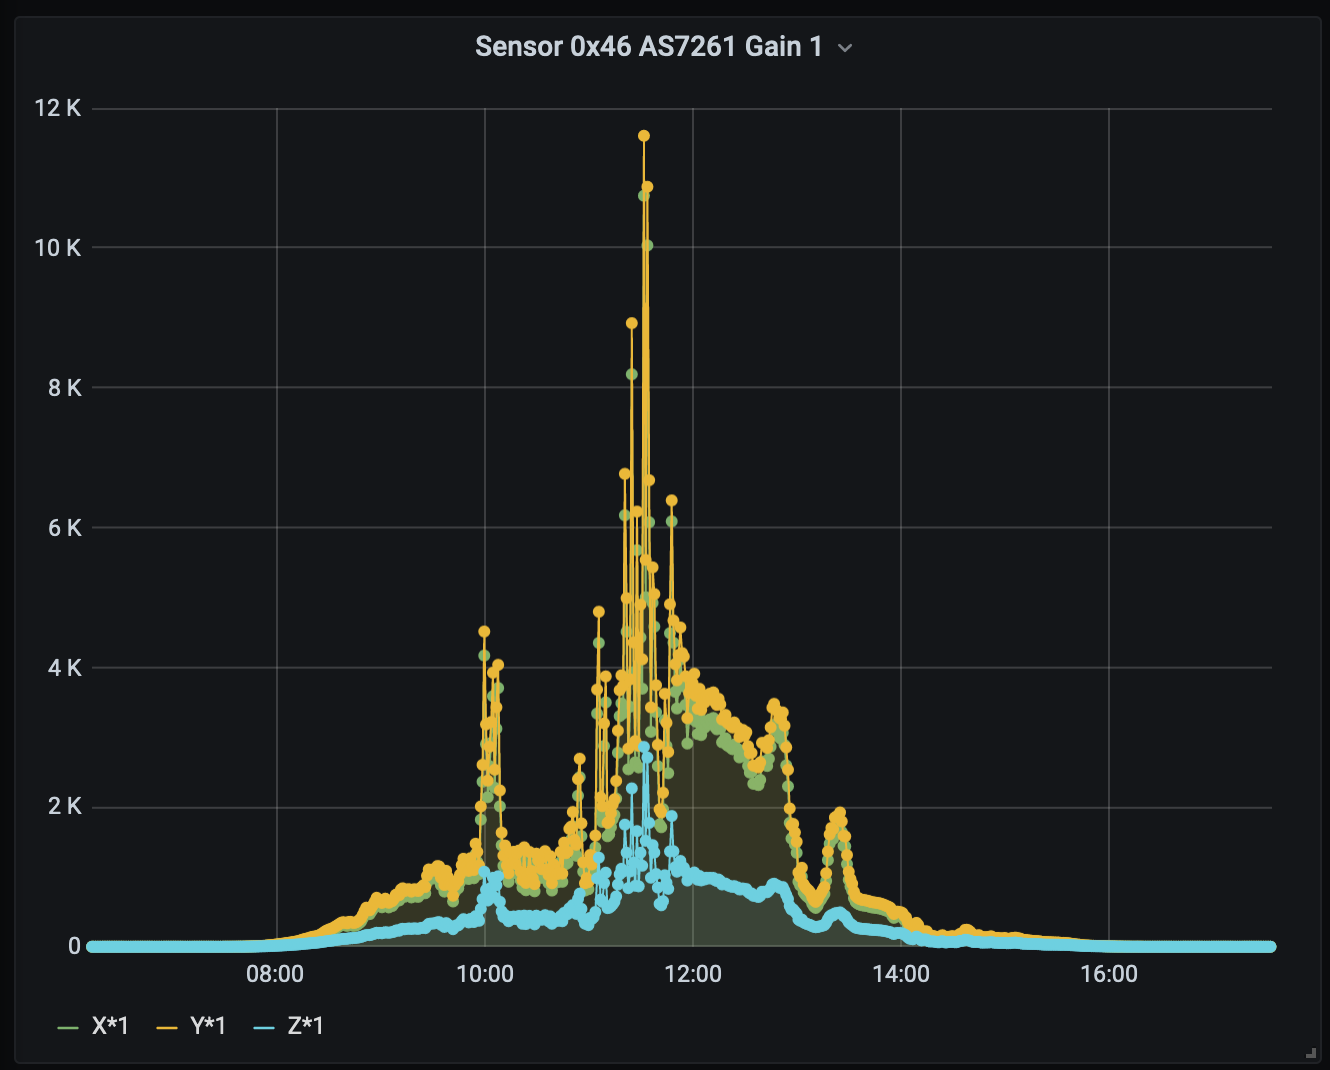
\includegraphics[width=\textwidth]{img/Grafana-Gain1}
    \caption{Gain 1 (3,7x)}
      \label{fig:Grafana_Gain1}
  \end{subfigure}
\end{figure}

\begin{figure}[H]
  \begin{subfigure}[b]{0.5\textwidth}
    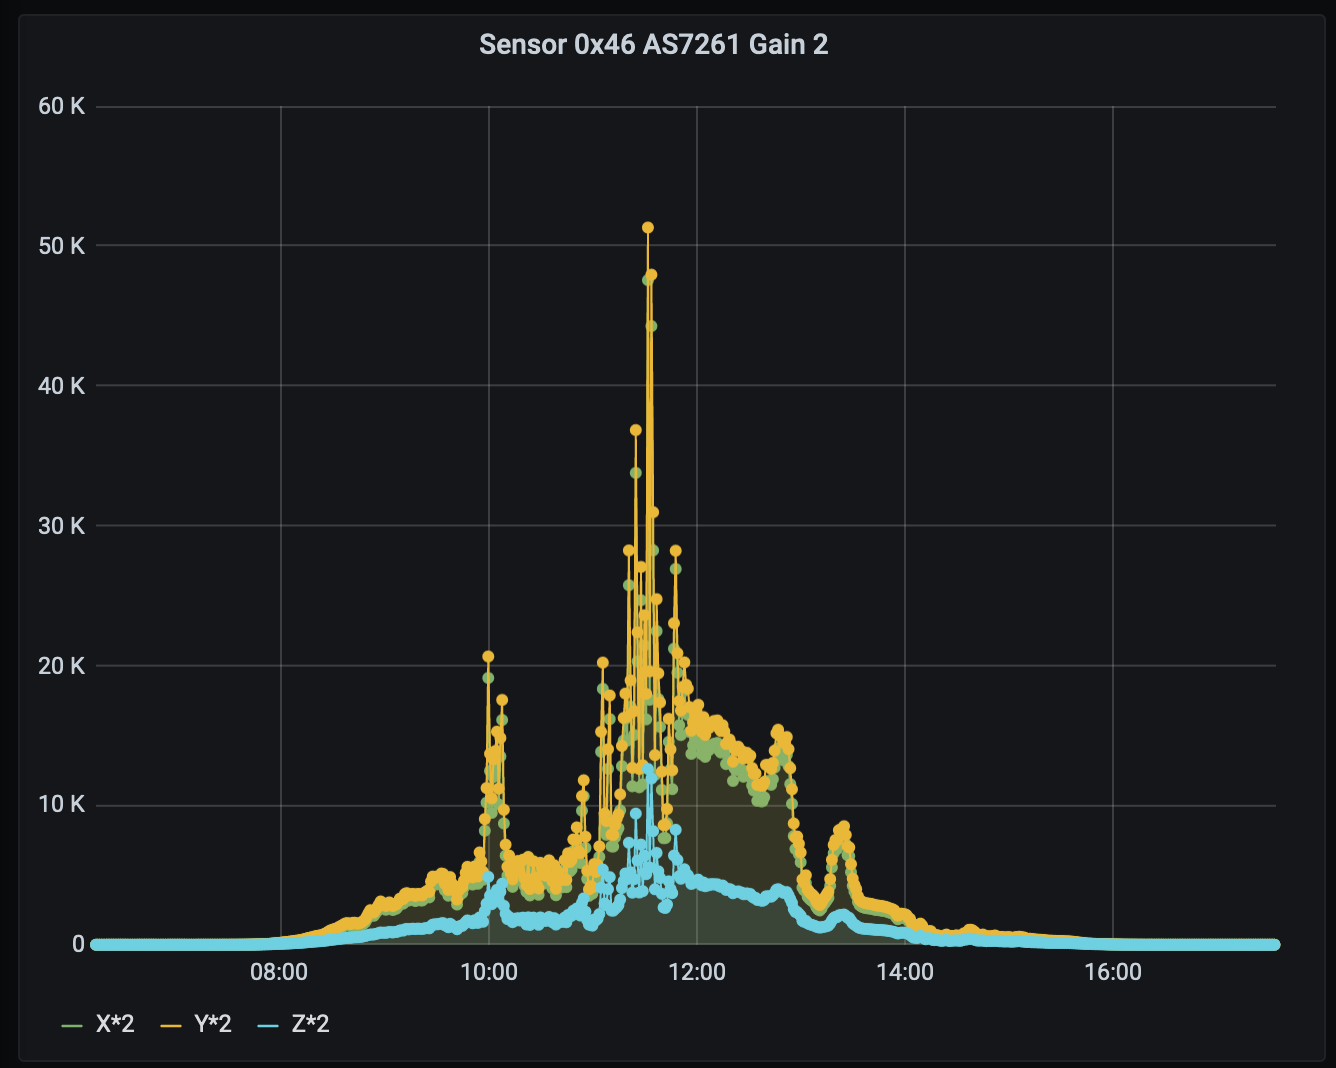
\includegraphics[width=\textwidth]{img/Grafana-Gain2}
   \caption{Gain 2 (16x)}
	\label{fig:Grafana_Gain2}
  \end{subfigure}
  %
  \begin{subfigure}[b]{0.5\textwidth}
    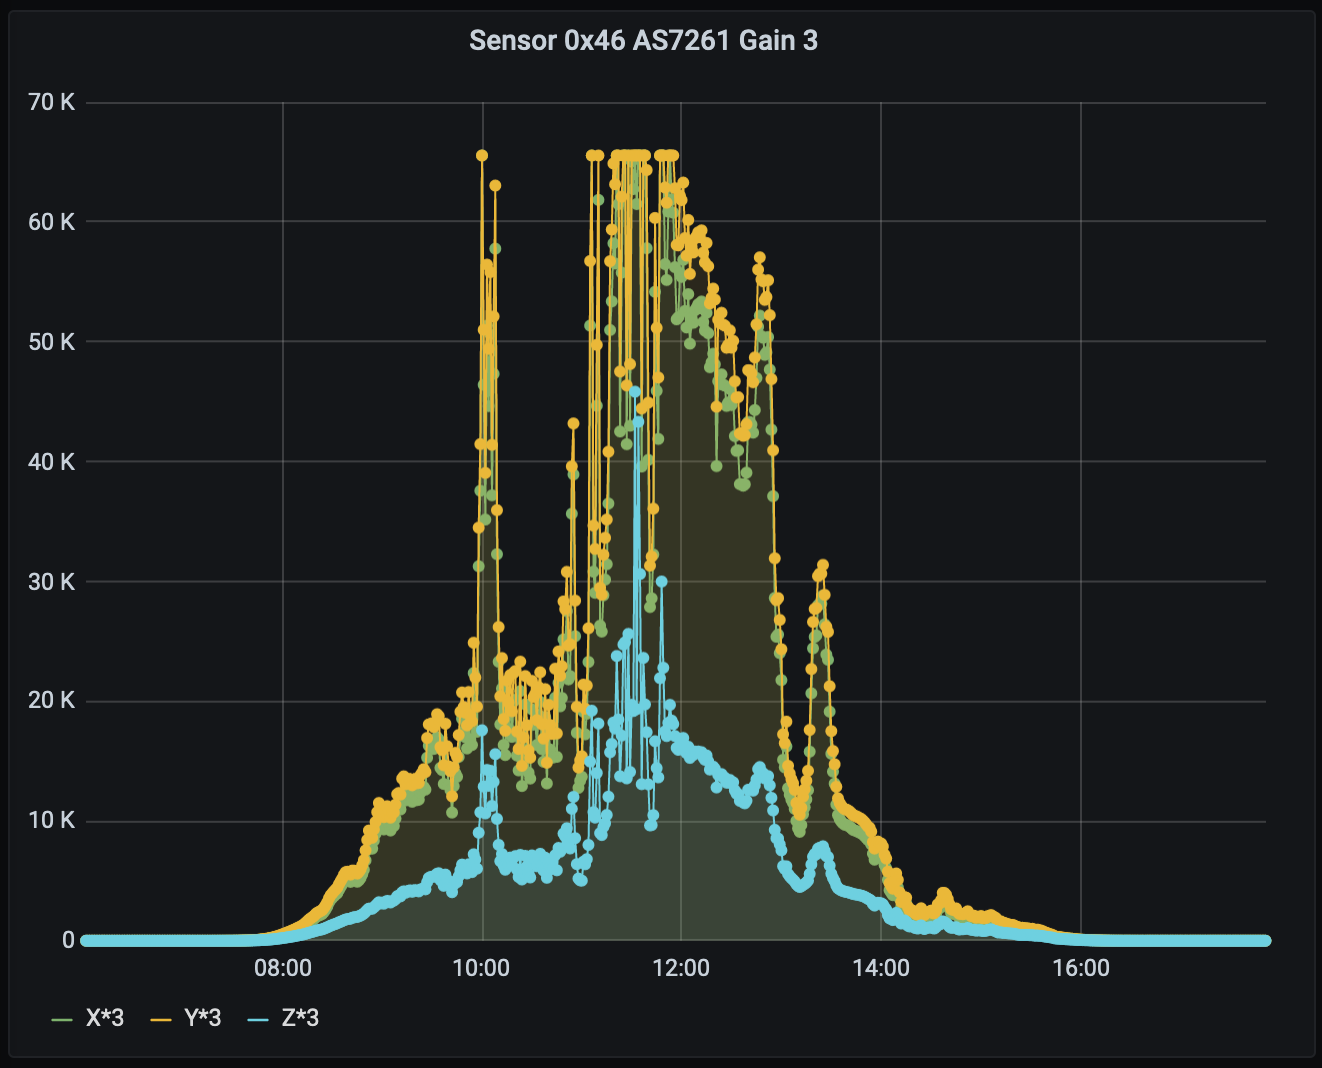
\includegraphics[width=\textwidth]{img/Grafana-Gain3}
	\caption{Gain 3 (64x)}
	\label{fig:Grafana_Gain3}
  \end{subfigure}
\end{figure}


\begin{figure}[H]
\centering
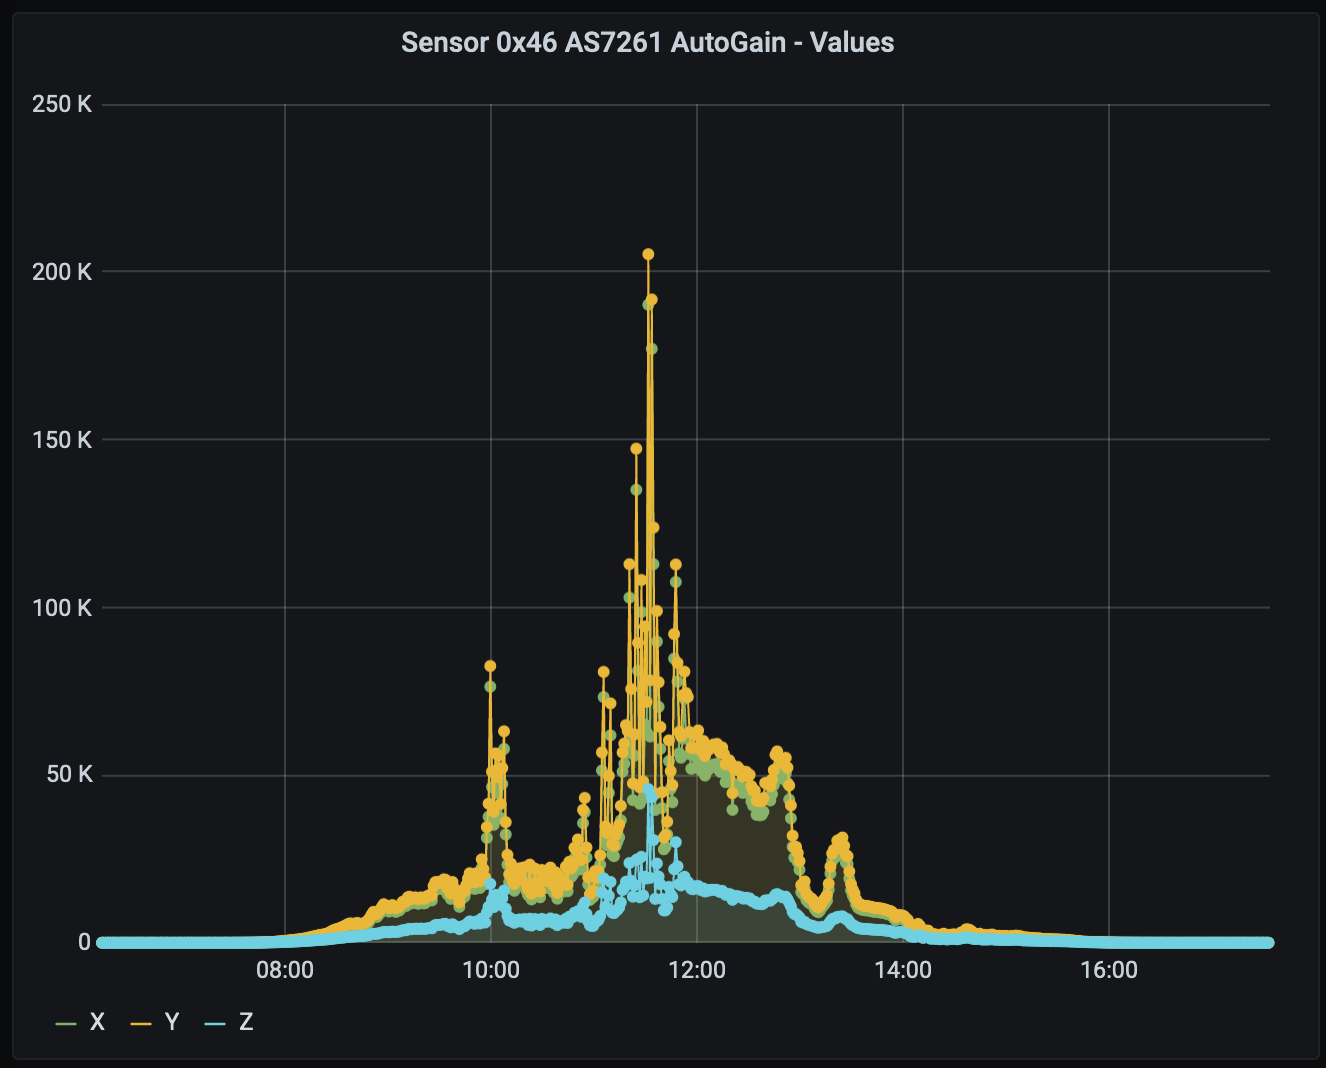
\includegraphics[width=0.6\textwidth]{img/Grafana-AutoGain}
\caption{AutoGain}
\label{fig:Grafana_AutoGain}
\end{figure}
